\begin{abstract}
Diffusion models have demonstrated impressive performance in generating high-quality videos from text prompts or images. 
However, precise control over the video generation process—such as camera manipulation or content editing—remains a significant challenge. 
Existing methods for controlled video generation are typically limited to a single control type, lacking the flexibility to handle diverse control demands.
In this paper, we introduce Diffusion as Shader (\methodname), a novel approach that supports multiple video control tasks within a unified architecture. 
Our key insight is that achieving versatile video control necessitates leveraging 3D control signals, as videos are fundamentally 2D renderings of dynamic 3D content. 
Unlike prior methods limited to 2D control signals, \methodname leverages 3D tracking videos as control inputs, making the video diffusion process inherently 3D-aware. This innovation allows \methodname to achieve a wide range of video controls by simply manipulating the 3D tracking videos. 
A further advantage of using 3D tracking videos is their ability to effectively link frames, significantly enhancing the temporal consistency of the generated videos.
With just 3 days of fine-tuning on 8 H800 GPUs using less than 10k videos, \methodname demonstrates strong control capabilities across diverse tasks, including mesh-to-video generation, camera control, motion transfer, and object manipulation. Codes and more results are available at \href{https://igl-hkust.github.io/das/}{https://igl-hkust.github.io/das/}.
% These results underscore \methodname’s potential to redefine the landscape of controlled video generation.
\end{abstract}


\keywords{}

\begin{teaserfigure}
\centering
  % \includegraphics[width=\textwidth]{}
  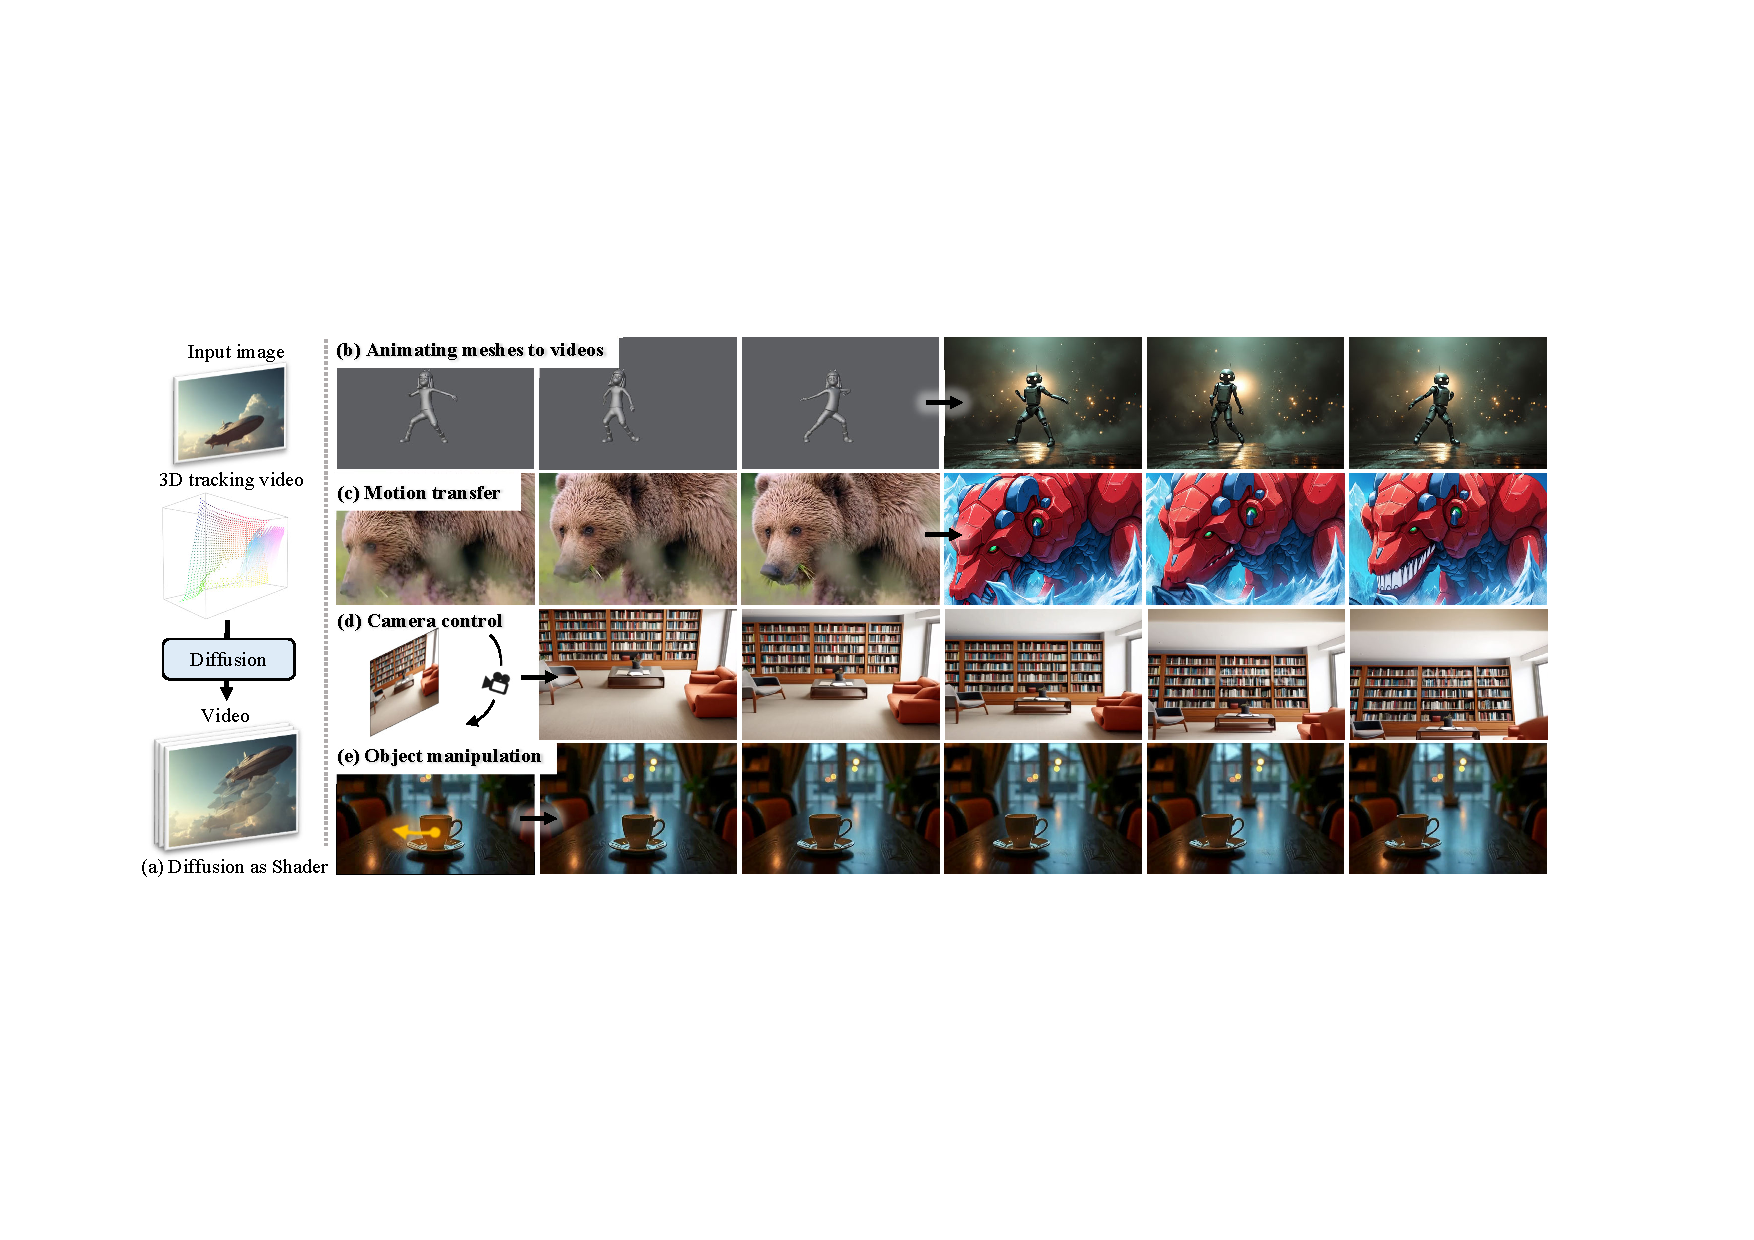
\includegraphics[width=\linewidth]{pictures/teaser.pdf}
  \vspace{-20pt}
  \caption{\textbf{Diffusion as Shader (\methodname)} is (a) a 3D-aware video diffusion method enabling versatile video control tasks including (b) animating meshes to video generation, (c) motion transfer, (d) camera control, and (e) object manipulation.}
  \label{fig:teaser}
\end{teaserfigure}

\maketitle